\begin{frame}{$\mathcal{T}$-Symmetric Honeycomb Band Insulators}
\vskip-1.5cm
\begin{columns}
\begin{column}[T]{0.65\textwidth}
%Famously
From considerations of graphene, a tight-binding honeycomb lattice model of fermions:

\bi
\item A spinless fermion has protected Dirac points
\bi
\item with $\mathcal{I}$ and $\mathcal{T}$ symmetry
\item NO featureless insulators at filling 1 on the honeycomb lattice with $\mathcal{T}$
%One way to say it: T guarantees m = m' where m and m' are the effective masses at the special momenta labeled K and K'
% On the otherhand, I guarantees m=-m' and with T broken gives a chern number \pm1. 
\ei 
\item<2-> Breaking  $\mathcal{T}$ leads to non-zero Chern number - $\mathbb{Z}$ invariant, QAHE 
%Haldane proposed using complex hopping amplitudes to do this in 1988 instead of a static magnetic field, QAHE -IQHE without net magnetic flux

%This situation can be exploited to make something new, by taking two copies.
\item<3-> Spinful fermions with spin-orbit couplings have two bands, with Chern numbers $\pm 1$.
%Net chern number and qhconductance is zero but there is quantum spin hall current
%Charlie Kane 2004
%2d topological insulator, edge is a kramers doublet in general
\item<3-> $\mathbb{Z}_2$ topological invariant 
\vskip-0.3cm
\ei
\end{column}
\begin{column}[T]{0.35\textwidth}
\only<1>{
    \begin{figure}
        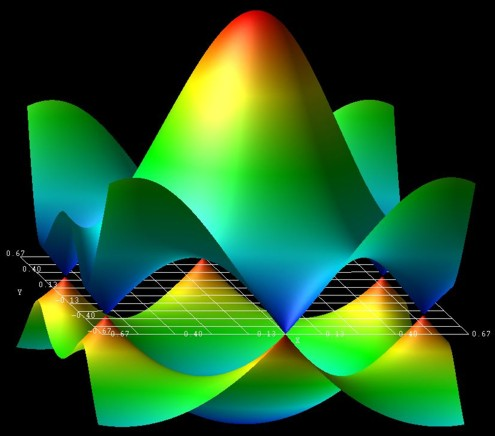
\includegraphics[width=\linewidth]{diagrams/grapheneband2.jpg}
        \caption{Dirac Points}
    \end{figure}
    \vskip-2cm
        \begin{figure}
        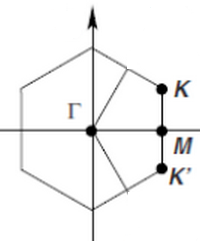
\includegraphics[width=\linewidth]{diagrams/kpoint.png}
        \caption{Brillouin Zone}
    \end{figure}
}
\only<2->{
\begin{figure}
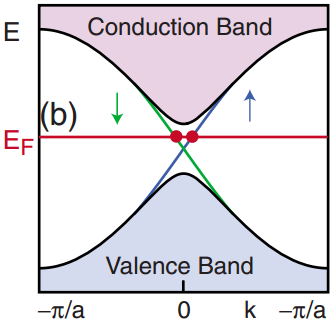
\includegraphics[width=\linewidth]{diagrams/helical_edge.png}
\caption{Helical Edge \footnotemark}
\end{figure}
\vskip-0.5cm
\bi 
\item $\mathcal{T}$-symmetric quantum spin-hall insulator.
%spin-hall conductance is non-zero
%edges can be gapped out by breaking T
\ei }
\end{column}
\end{columns}
\footnotetext[2]{
\citep{Hasan2010-fq}} 
\end{frame}